\documentclass[12pt, a4paper]{scrreprt}
\usepackage[utf8]{inputenc}
\usepackage[ngerman]{babel}
\usepackage[bookmarksnumbered]{hyperref}
\usepackage{graphicx}
\usepackage{keystroke} %Keyboardsymbole

\begin{document}
\begin{titlepage}
\titlehead{
	\begin{minipage}[c][5cm][c]{5cm}
	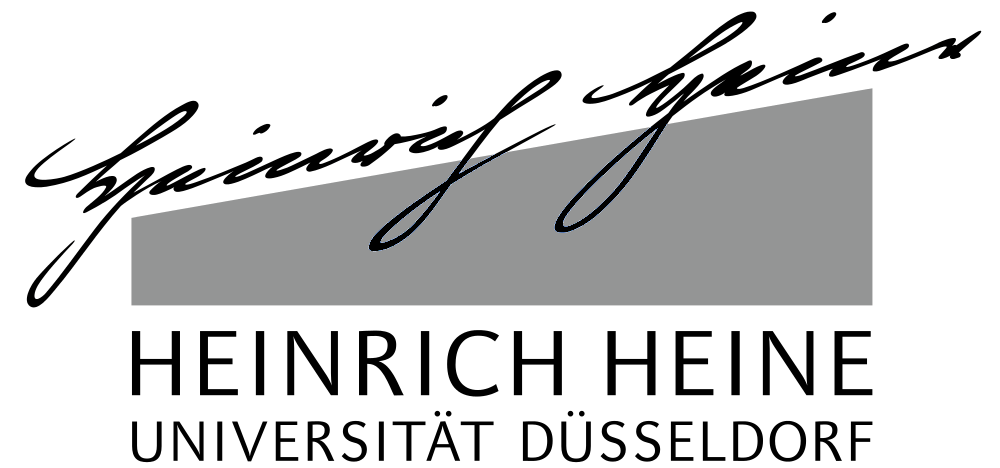
\includegraphics[width=48mm]{logo2}
	\end{minipage}
	\hfill
	\begin{minipage}[c][5cm][c]{10cm}
	\begin{flushright}
	\textbf{Universität Düsseldorf\\Mathematisch-Naturwissenschaftliche Fakultät\\Institut für Informatik\\Dozent:} PD Dr. Wilfried Linder
	\end{flushright}
	\end{minipage}
}
\subject{Benutzerhandbuch}
\title{Dungeon Crawler 	
	\begin{minipage}[c][1cm][c]{1cm}
	
\includegraphics[width=10mm]{Icon}
	\end{minipage}}
\subtitle{Programmierpraktikum im Sommersemester 2013}
\author{Michael Beurskens\\ Robin Thüs\\ Ruslan Curbanov}
\publishers{Gruppe 22}
\maketitle
\end{titlepage}
\tableofcontents
\chapter{Einleitung}
\section{Vorwort und Systemanforderungen}
\subsection*{Gesundheitsschutz}
\begin{itemize}
\item Legen Sie zum Schutz Ihrer Gesundheit eine Pause von 15 Minuten pro Spielstunde ein.
\item Spielen Sie nicht wenn Sie müde sind oder nicht genug Schlaf hatten.
\item Spielen Sie immer in einem gut beleuchteten Raum und setzen Sie sich so weit vom Bildschirm entfernt, wie es das Kabel Ihrer Eingabegeräte zulässt.
\item Bei einem sehr kleinen Prozentsatz von Personen kann es zu epileptischen Anfällen kommen, wenn sie bestimmten Lichteffekten oder Lichtmustern in ihrer täglichen Umgebung ausgesetzt sind.
\item Manchmal wird bei diesen Personen ein epileptischer Anfall ausgelöst, wenn sie Computerspiele spielen. Auch Spieler, die zuvor noch nie einen Anfall hatten, können an bisher nicht erkannter Epilepsie leiden. Falls Sie an Epilepsie leiden, suchen Sie Ihren Arzt auf, bevor Sie Computerspiele betreiben. Sollten bei Ihnen eines der folgenden Symptome auftreten (Schwindelgefühl, veränderte Sehkraft, Muskelzuckungen, jegliche Art von unkontrollierter Bewegung, Bewusstseinsverlust, Desorientierung und/oder Krämpfe), so brechen Sie das Spiel sofort ab und suchen einen Arzt auf.
\end{itemize}
\subsection*{Spielstart}
Vielen Dank, dass Sie sich für unsere neuste Entwicklung des Computerspiele-Zeitalters entschieden haben. Ich darf stolz verkünden, dass Sie mit diese Entscheidung eine hervorragende Wahl getroffen haben. Dungeon Crawler 2013 (Gruppe 22) wird nach unseren Prognosen das beliebteste Spiel des Jahres 2013!\\
\begin{enumerate}
\item Beachten Sie zunächst die Systemanforderungen, bevor Sie das Spiel Installieren.
\item Schalten Sie Ihren Computer ein und installieren das Spiel.
\item Starten Sie das Spiel mit \textit{Gruppe22.exe} (Server: \textit{DungeonServer.exe}).
\end{enumerate}
\subsection*{Systemanforderungen}
Bei der Entwicklung wurde besonders viel Wert auf Kompatibilität zu verschiedenen Geräten bzw. Systemen gelegt. Die hier zugrunde liegende Version ist jedoch nur unter Windows (ab XP bzw. unter .NET-Framework) lauffähig.\\
Beachten Sie: Das Spiel nutzt die Grafikbibliotheken \textit{OpenGL} (und \textit{OpenAL}), Ihre Grafikkarte sollte dies also unbedingt unterstützen.\\\\
Und sonst: Jedes halbwegs moderne Rechner tut's ;)
\section{Befehlsliste und Steuerung}
\textbf{\textit{Hinweis:}} Im folgenden wird mit dem Begriff \textit{Hauptmenü} das \textit{Pausenmenü} bezeichnet, da es sich in diesem GUI-System um das selbe Menü handelt.
\begin{center}
\begin{tabular}[here]{|l|l|}
\hline
Bewegen & \textit{Maus in Zielrichtung halten und linke Maustaste gedrückt halten}\\ \hline
Aktion & \textit{linke Maustaste drücken und halten (auf aktionsfähigem Objekt)}\\ \hline
Angriff & siehe Aktion\\ \hline
Sekundärwaffe & \textit{Leertaste \Spacebar}\\ \hline
\multicolumn{2}{|c|}{Menüsteuerung und sonstige Befehle}\\ \hline
Pausenmenü & \Esc\\ \hline
Chateingabe & \keystroke{T}\\ \hline
Charakter & \keystroke{C}\\ \hline
Inventar & \keystroke{I}\\ \hline
Fähigkeiten & \keystroke{S}\\ \hline
\end{tabular}
\end{center}
Außerdem stehen Ihnen Drag-and-Drop mit Maus für Objekte- und Minimap-Verwaltung bzw. Verschiebung zur Verfügung.
\clearpage
\section{Prolog}
Guten Tag, wir haben neue Abenteuer für Sie in diesem letzten Dungeon Crawler 2013.\\\\
Sie befinden sich in einem Labyrinth, bestehend aus mehreren Räumen und Ebenen.\\
Das Ziel ist es die höchste Ebene zu erreichen und damit in die Freiheit zu entkommen, denn Sie sind tief unter der Erde in einer gefährlichen Umgebung voller Irrwege. Es wird wichtig sein einen guten Orientierungssinn zu besitzen oder sich geschickt anzustellen, denn je mehr Sie herumirren desto gefährlicher wird es für Sie. Mit jedem Level bzw. jeder Ebene steigert sich der Schwierigkeitsgrad (z.B. werden die Gegner stärker, der Sichtradius immer kleiner) und auf jeder Ebene wartet eine besondere Überraschung! Ein spezieller Boss-Gegner, der alles unter Kontrolle hat und Acht darauf gibt das keiner die Ebene wechselt. Sie sollten auch auspassen wohin Sie treten, es gibt nämlich Fallen die nicht zu unterschätzen sind. Um erfolgreich zu sein ist es unbedingt erforderlich Erfahrung durch Kämpfe zu sammeln und achten Sie auch auf dinge die sonst so herumliegen. Ein ausgeklügeltes Gameplay-System erlaubt Ihnen zusätzlich die Übersicht und Verwaltung über Ihr Inventar und sonstigen Charaktereigenschaften. Sie sollten die Kraft der Magie nicht auf die leichte Schulter nehmen, diese kann sehr hilfreich sein und wenn es mal knapp wird gibt es keine bessere Hilfestellung. Schließlich runden einige interaktive NPCs das Spiel ab. Sie können zum Beispiel den Shop besuchen um sich dort auf die nächste Schlacht vorzubereiten. Und keine sorge falls Sie nicht genug Geld besitzen, die Moralentscheidungen sind ganz Ihnen überlassen.\\\\
Viel Erfolg beim Kampf in die Freiheit
\section{Besetzung}
\subsection*{Hauptcharakter}
Der Hauptcharakter (Spieler) ist ein furchtloser Ritter, der immer zu kämpfen bereit ist.
\subsection*{NPCs}
Es gibt verschiedene NPCs, interaktive(Dialog/Quest) und Shop.
\subsection*{Skelett}
Der erste und älteste Gegner. Nicht sehr intelligent.
\subsection*{Die Spinne}
Eine beengstigende Kreatur, man sollte ihre Schnelligkeit und Intelligenz nicht unterschätzen.
\subsection*{Der Kobold}
Diese Art von Gegner können nervig sein.
\subsection*{Der Drache}
Achten Sie auf die großen Zähne.
\subsection*{Bossgegner}
In jedem Level erwartet Sie ein Raum mit dem Bossgegner, Sie müssen ihn bezwingen um an die Schlüssel heran zu kommen.
\section{Schauplätze}
Jeder Raum hat seinen eigenen Scharm, und auch wenn alle Räume ähnlich aussehen, gibt es doch ein paar Worte zu sagen.\\
Die Räumen und Ihre gegenseitige Abhängigkeit sind zufällig, folgen jedoch gewissen Einschränkungen, die dazu dienen den Spielspaß zu sichern. Ihnen wird aufgefallen sein, das die Gestaltung der Umwelt äußerlich variiert (beachte Sie dazu auch die Größe der Grafiken von ca. 600MB), doch auch die Geometrie der Räume wird je nach Level angepasst. Je höher Sie kommen desto weniger Wände werden im Raum stören, das liegt daran das die Oberfläche immer näher kommt und das Labyrinth an dichte verliert. Jedoch sind Sie dadurch ein leichteres Ziel für die verbitterten Kreaturen der Unterwelt. Sie sollten das also in Ihrer Strategie unbedingt mit einbeziehen.
\chapter{Einrichten des Spiels}
\section{Hauptmenü}
\begin{figure}[h]
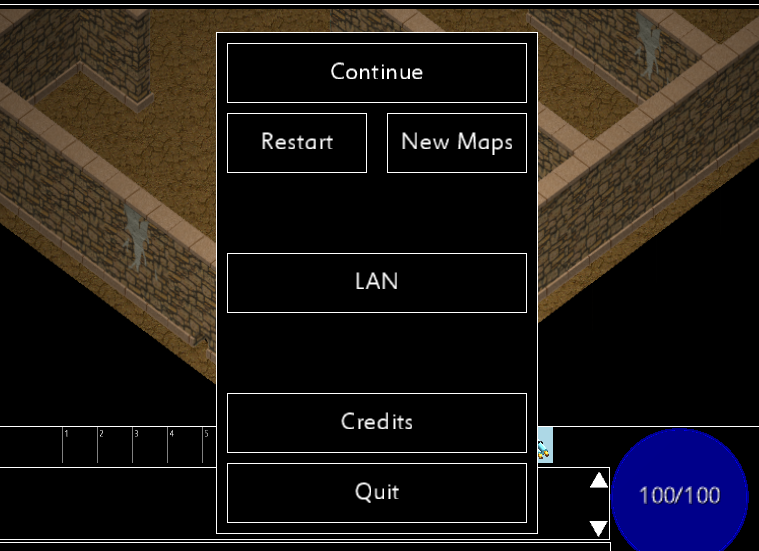
\includegraphics[width=\textwidth]{img/menu}
\caption{Hauptmenü des Spiels.}
\end{figure}
In der obigen Abbildung sehen Sie das Haupt- bzw. Pausenmenü. Dieses ist das wichtigste Menü, dort gibt es folgende Möglichkeiten:
\begin{itemize}
\item \textit{Continue}: Schließt das Hauptmenü wieder und das Spiel wird fortgesetzt. Beachten Sie, dass im Multiplayermodus das Spiel weiterläuft, auch wenn Sie das Pausenmenü aufgerufen haben.
\item \textit{Restart}: Dies startet das Spiel neu.
\item \textit{New Maps}: Da die Karte in diesem Spiel zufällig erzeugt wird, besteht die Möglichkeit, dass Sie sich eine neue Welt generieren lassen können, dann fängt das Spiel allerdings von neu an und Sie müssen wieder alle Ebenen bezwingen.
\item \textit{LAN}: Dieser Button öffnet die Mehrspieler-Optionen, die zur Verfügung stehen. (Nur für LAN Spiele vorgesehen)
\item \textit{Credits}: Hier können Sie die Credits-Informationen einsehen.
\item \textit{Quit}: Dieser Punkt beendet das Spiel.
\end{itemize}
\section{Optionen}
\begin{figure}[h]
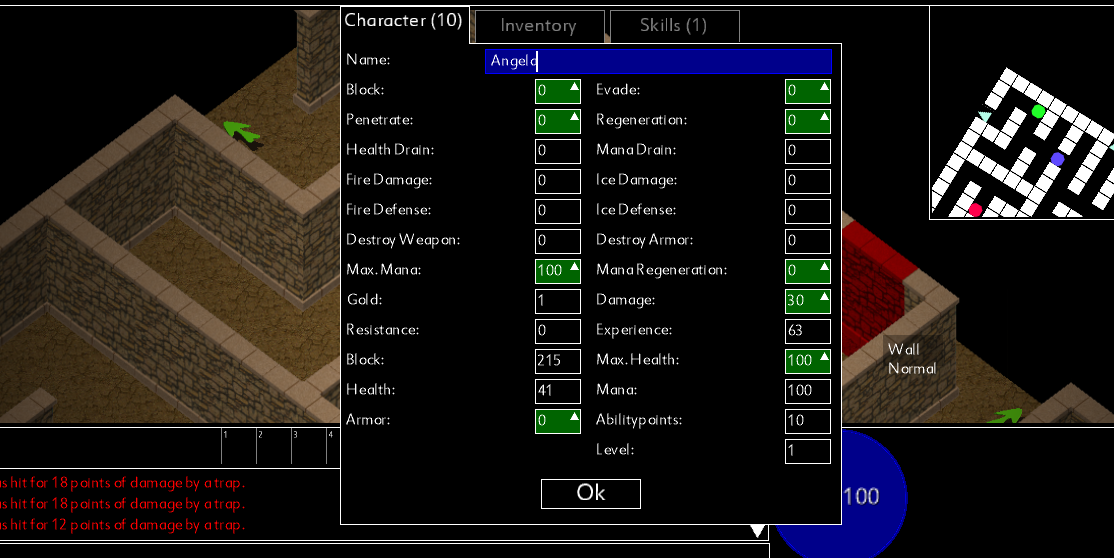
\includegraphics[width=\textwidth]{img/character}
\caption{Optionsfenster für die Charaktereigenschaften des Spielers.}
\vspace{1cm}
Hier sehen Sie Ihren Charakter, dieser kann angepasst werden in dem Sie verschiedene Eigenschaften Ihrer Figur durch erhöhen der zahl ausprägen. Dazu sehen Sie in Klammern (bzw. weiter unten) die sog. Abilitypoints, welche Sie auf die Eigenschaften verteilen. Auch dieser Punkt hilft Ihnen im Spiel und entscheidet über die Schwierigkeitsstufe, es ist somit empfehlenswert die für Sie wichtigen Eigenschaften stets zu aktualisieren.
\end{figure}
\begin{figure}[h]
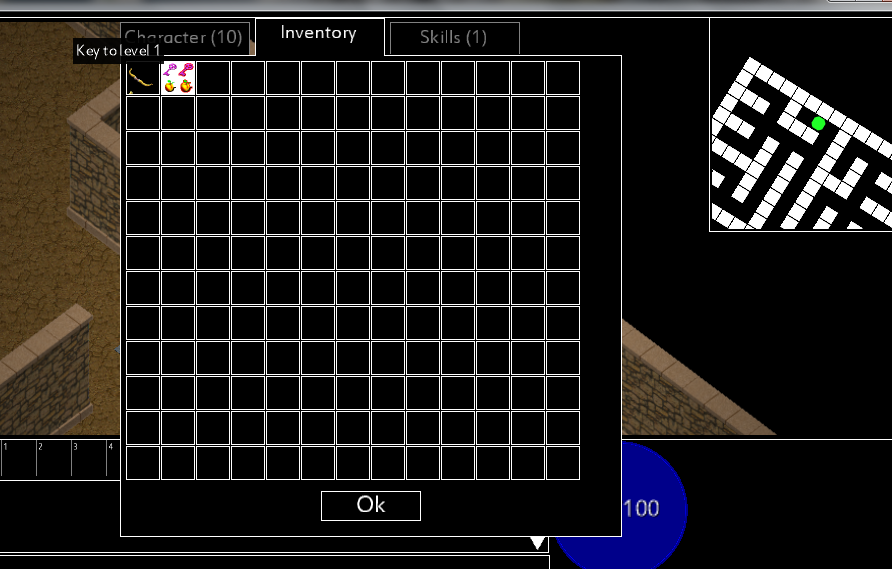
\includegraphics[width=\textwidth]{img/inventory_havekey}
\caption{Optionsfenster für das Inventar des Spielers.}
\vspace{1cm}
Dies ist Ihre Inventar-Liste, Sie sehen dort alles was Sie besitzen. Also Objekte die Sie aufgehoben haben wie Waffen, Rüstung und spezielle Objekte. Auch den Schlüssel zu einem Level finden Sie dort.
\end{figure}
\begin{figure}[h]
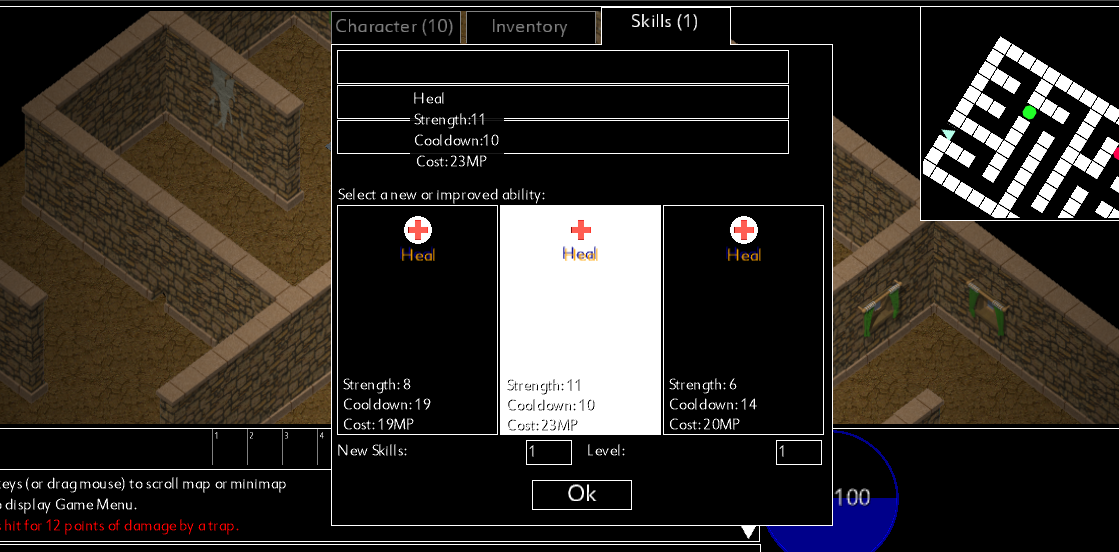
\includegraphics[width=\textwidth]{img/skills}
\caption{Optionsfenster für die Fähigkeiten des Spielers.}
\vspace{1cm}
Vergessen Sie nicht sich mit Fähigkeiten auszurüsten, diese werden sich als große Erleichterung offenbaren, wenn Sie sonst immer an einer Stelle hängen bleiben. Fähigkeiten hängen stark von Ihrer Erfahrung im Kampf ab.
\end{figure}
\chapter{Gameplay und Anzeigesysteme}
\begin{figure}[h]
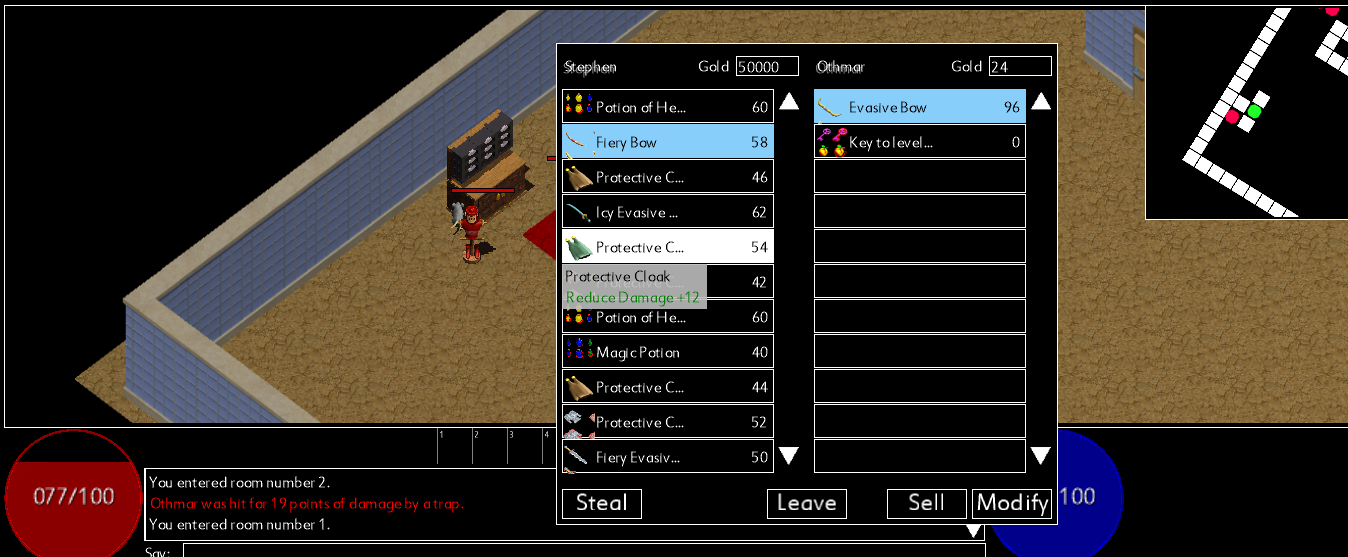
\includegraphics[width=\textwidth]{img/shop_system}
\caption{Der freundliche Shop.}
\vspace{1cm}
Das Shopsystem ist ein geben und nehmen. Ihnen stehen beide Möglichkeiten zu Verfügung. Entscheiden Sie selbst ob Sie mit dem Händler fair bleiben wollen oder nicht, wenn Sie ihn jedoch zu oft verärgern und bestehlen kann es böse für Sie enden. Entscheiden Sie!
\end{figure}
\begin{figure}[h]
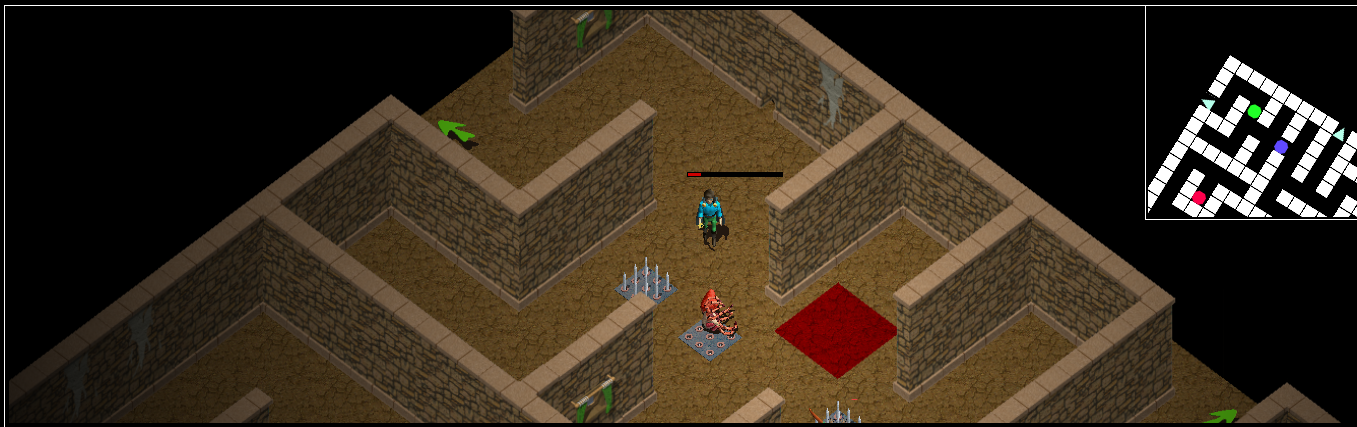
\includegraphics[width=\textwidth]{img/trap_enemy(dead)_transportarrow_objekt(blue)}
\caption{Fallen, Feinde(tot), Raumwechsel, Objekte(Minimap).}
\vspace{1cm}
In dieser Abbildung sieht man mehrere Dinge auf die ich eingehen möchte.
\begin{enumerate}
\item Fallen sind intelligenter als auf diesem unbewegten Bild zu erkennen, je öfter Sie ihnen auszuweichen versuchen, desto schneller werden sie. Das wichtigste Prinzip: Bleiben Sie auf keinen Fall auf einer Falle stehen, es sei den Sie möchten zum letzten Checkpoint zurückkehren.
\item Wie sie sehen werden auch Ihre Feinde von Fallen verletzt und der Körper bleibt dann auch auf dem Boden liegen.
\item Dabei lassen die Kreaturen das Inventar auf dem Boden fallen und Sie können die Objekte einsammeln.\\
Achten Sie auch Auf die Minimap(oben rechts), die Ihnen bei der Orientierung hilft. Die weißen Vierecke sind Wände. An der Kreisen bzw. Farben erkennen Sie verschiedene Objekte. Rot steht für Gegner/anderer Spieler, Blau für ein Item, grün markiert ihren aktuellen Standort und die türkisfarbenden Pfeile stehen für den Raumwechsel.
\end{enumerate}
\end{figure}
\begin{figure}[h]
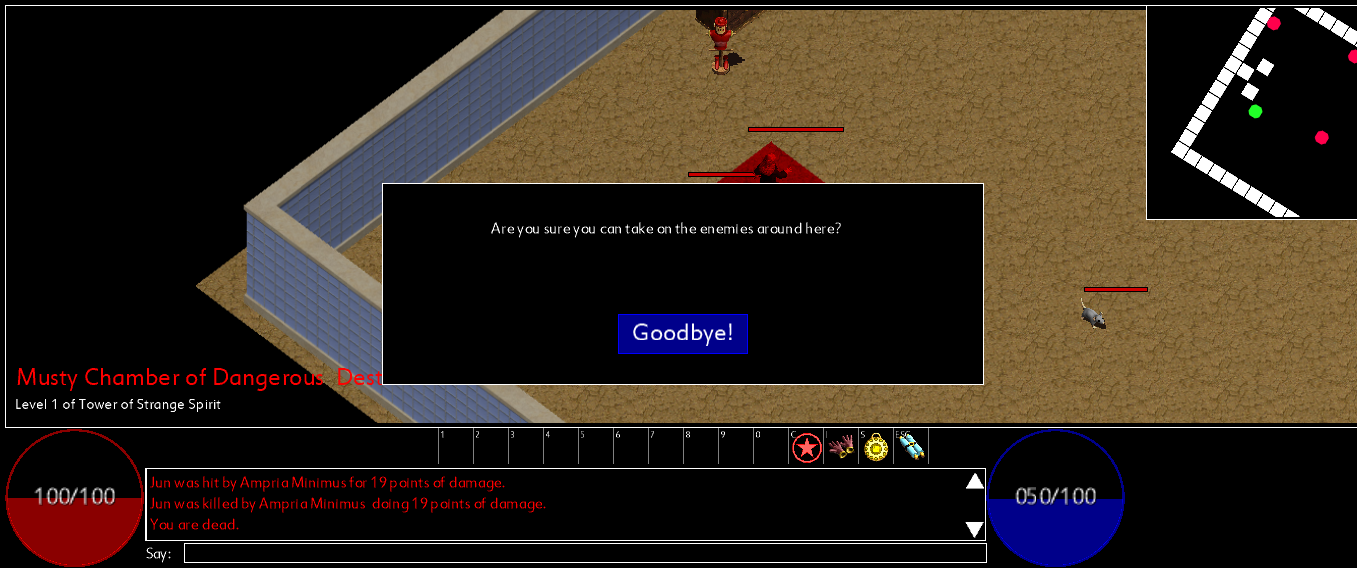
\includegraphics[width=\textwidth]{img/dialog_with_NPC}
\label{fig:chat}
\caption{Chatsystem und untere Anzeigeleiste, Dialog mit NPCs und Quests.}
\vspace{1cm}
Auf diesem Bild sehen Sie ein Dialog mit einem NPC. Auf diese Weise sollen nicht nur unterhaltsamer Texte vermittelt werden sondern auch die Quests. Außerdem soll an der Stelle das Anzeigesystem (unten) erläutert werden. Die zwei Kreise links und rechts zeigen den aktuellen Stand der Lebenspunkte und Mana. In der Mitte befindet sich der Schnellzugriff für die Optionsmenüs und ausgewählte Objekte die dynamisch (via Drop and Drag) verwaltet werden können. Direkt drunter ist ein Textfeld wo Nachrichten (Chat), Hinweise zum Spiel und Ereignisbeschreibungen angezeigt werden. ganz unten ist das Texteingabefeld für den Chat im Multiplayermodus.
\end{figure}
\chapter{Multiplayer}
\section{Die Lobby}
\begin{figure}[h]
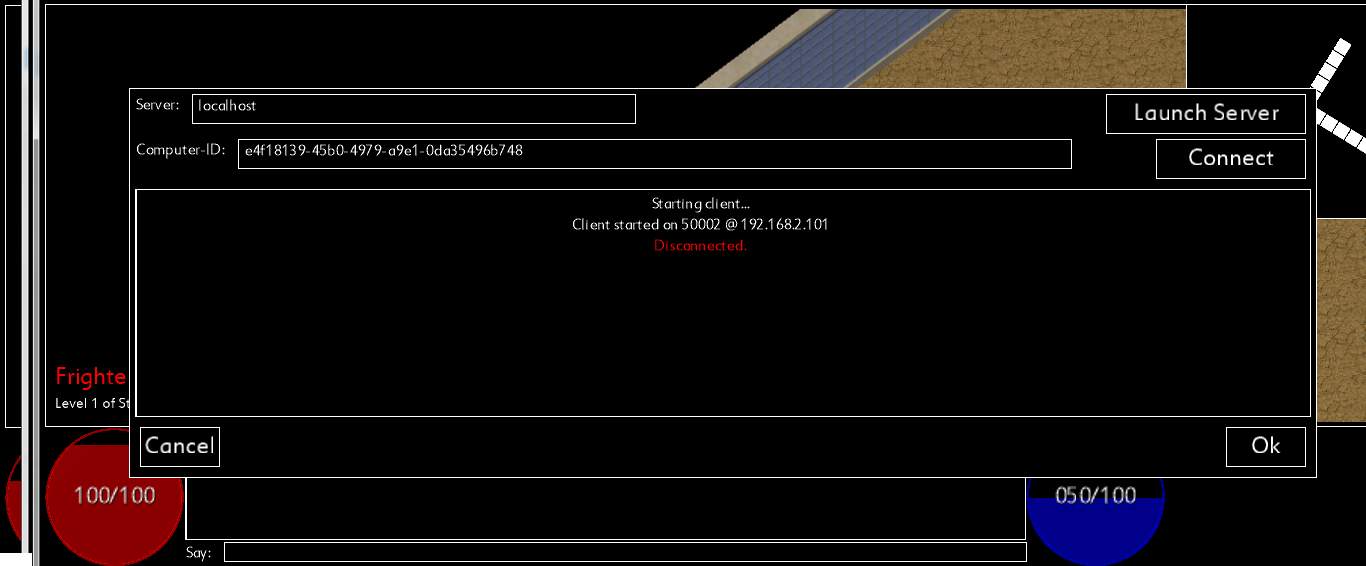
\includegraphics[width=\textwidth]{img/multiplayer}
\caption{Lobby.}
\vspace{1cm}
Hier sehen Sie die Lobby für den Mehrspielermodus. Sie sehen dort intuitiv ob ein Server im lokalen Netzwerk gesichtet wurde. Sie können sich dann mit diesem verbinden um am Spiel teilzunehmen. Es gibt jedoch auch die Möglichkeit einen Server selbst zu starten, falls noch keiner im Netzwerk angemeldet ist.
\end{figure}
\subsection*{Das Chatsystem}
Das Chatsystem wurde bereits in Kapitel 3, Abb. \ref{fig:chat} vorgestellt.
\chapter{Speichern und Laden}
\section*{Checkpoints}
\begin{figure}[h]
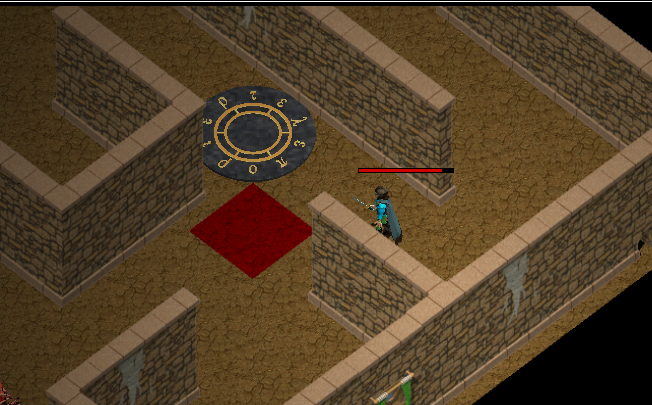
\includegraphics[width=0.3\textwidth]{img/checkpoint(unchecked)}
\caption{Unchecked.}
\end{figure}
\begin{figure}[h]
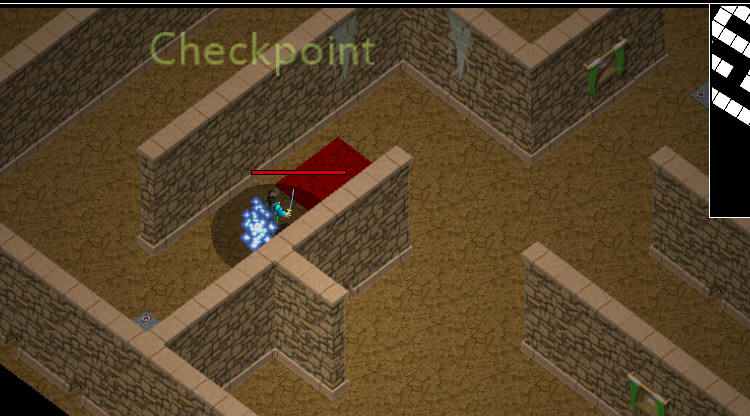
\includegraphics[width=0.3\textwidth]{img/checkpoint(checked)}
\caption{Checked.}
\end{figure}
Sie haben in manchen Räumen die Checkpoints, wenn Sie sterben stehen insgesamt 3 Versuche zur Verfügung es ab dem letzten Checkpoint nochmal zu versuchen.\\
Außerdem ist noch zu erwähnen, dass das Spiel automatisch (im Hintergrund) speichert, dies ist jedoch eher ein technisch relevantes Detail. Geladen wird beim Start des Spiels ebenfalls automatisch.
\chapter{Lizenzbedingungen}
Dungeon Crawler 2013\\\\
Developed by Group 22\\\\
*********************************\\\\
Music: Video Dungeon Crawl by Kevin MacLeod is licensed under a CC Attribution 3.0\\\\
\url{http://incompetech.com/music/royalty-free/index.html?collection=029}\\\\
Graphics: Tile Graphics by Reiner Prokein\\\\
\url{http://www.reinerstilesets.de/de/lizenz/}
\chapter{Support}
Aus finanziellen Gründen können wir leider keine Hotline zur Verfügung stellen, bei Fragen wenden Sie sich bitte an die Entwickler.\\\\
\textbf{\textit{Hinweis:}} Das zugrunde liegende Bildmaterial kann von einer aktuelleren Version des Spiels abweichen, die Beschreibungen und Instruktionen bleiben jedoch richtig!
\end{document}